%%%%%%%%%%%%%%%%%%%%%%%%% Design %%%%%%%%%%%%%%%%%%%%%%%

\section{Design}

In this section we will explain the most important design decisions and the
reasons why they were taken. We will also go into detail in the most
remarkable characteristics.


%% Intro
\subsection{Bundles design}
\label{subsec:bundles-design}
One of the first and most important decisions is how to divide the
functionality into components. Having the requirement of using OSGi, it seems
natural to use a bundle as the notion of component.
The final design consists of four bundles:

\begin{itemize}
	\item \verb|RepositoryManager|, which has the following responsibilities:
	  	\begin{itemize}
	        \item Offer services to share applications.
	        \item Offer services to retrieve applications.
	        \item Storage of shared applications.
	        \item Offer services to search applications by criteria.
	        \item Offer services to search applications by similarity.
          \end{itemize} 
          
	\item \verb|TagManagerBackEnd|, which has the following responsibilities:
	  	\begin{itemize}
	        \item Offer services to add and delete public and community tags.
	        \item Offer services to retrieve those tags in different and flexible
	        ways.
          \end{itemize} 
          
	\item \verb|TagManagerNode|, which has the following responsibilities:
	  	\begin{itemize}
	        \item Offer services to add and delete private tags.
	        \item Offer services to retrieve those tags in different and flexible
	        ways.
        \end{itemize} 
          
	\item \verb|ApplicationManager|, which is responsible of the interaction with
	the user, and connects with the proper bundles to satisfy his requests.
      
\end{itemize}

The components diagram in Figure \ref{img:bundles-components-main} shows the
connection between all of them through its interfaces\footnote{The connection
with the rest of ASTRA bundles is omitted for simplicity reasons, but it will 
be discussed in the section where every bundle is explained.}:

\begin{figure}[h!]
 \begin{center}
 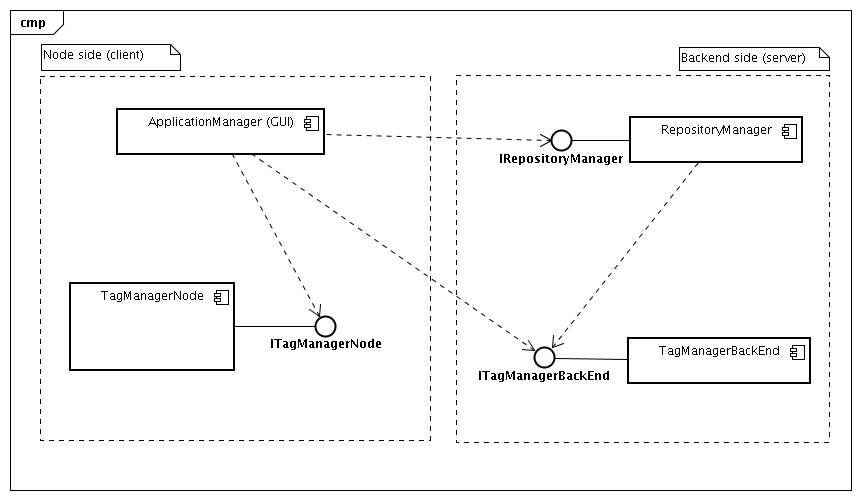
\includegraphics[scale=0.4]{diagrams/BundlesComponentsDiagram.png}
  \caption{\label{img:bundles-components-main}Relationships between the bundles
  developed for this project (components diagram)}
 \end{center}
\end{figure}

Sections \ref{subsec:repository-design}, \ref{subsec:tmbe-design},
\ref{subsec:tmn-design} and \ref{subsec:am-design} explain the most important
features of each of them.

%%%%%%%%%%%%%%% RepositoryManager %%%%%%%%%%%%%%%%%%%%%%%%%

\subsection{RepositoryManager}
\label{subsec:repository-design}

Since one of the most important goals of the project is the need of allowing
the users to share and retrieve applications, \verb|RepositoryManager| is one of
the key pieces of the project.
This bundle is executed in the Backend (server-side), and it offers a clear
interface to make its services available for the rest of the bundles
in ASTRA.

In this section we will explain the process we followed to perform its design.
Some of the trickiest implementation details about this bundle are explained
in Section \ref{sec:implementation}.

\subsubsection{Connection with other bundles}
\label{subsubsec:connections-rm}
The first step consists of analyzing the relationship between this bundle and
the rest of bundles in ASTRA.
Taking into account the requirements stated in Section \ref{sec:requirements}
and the analysis performed in Sections \ref{subsec:rm-use-cases} and
\ref{subsec:searching-use-cases}, we needed to make use of the services of  the
following bundles:

\begin{itemize}
  \item \verb|CommunityManager|: Necessary to retrieve information about the
  relationship between users, their communities and the applications. I.e.: to
  assure the visibility of certain application taking into account the
  communities joined for an user who is going to retrieve applications.
  \item \verb|TagManagerBackEnd|\footnote{The design of this bundle is explained
  in Section \ref{subsec:tmbe-design}}: Necessary to analyze the tags in order to
  construct the index of the search engine.
  \item \verb|EventsManager|: Necessary to keep track of the events produced
  in\\ \verb|TagManagerBackEnd|, in order to keep the index of the search engine updated.
  I.e: new tags or tags that have been deleted.
  \item \verb|PersistencyManager|: Necessary to store permanently all the data
  into the database. Using its services, we assure the robustness of the system.
\end{itemize}

The Figure \ref{img:rm-components} shows graphically the relationship between
\verb|RepositoryManager| and the rest of components through its interfaces.

\begin{figure}[h!]
 \begin{center}
 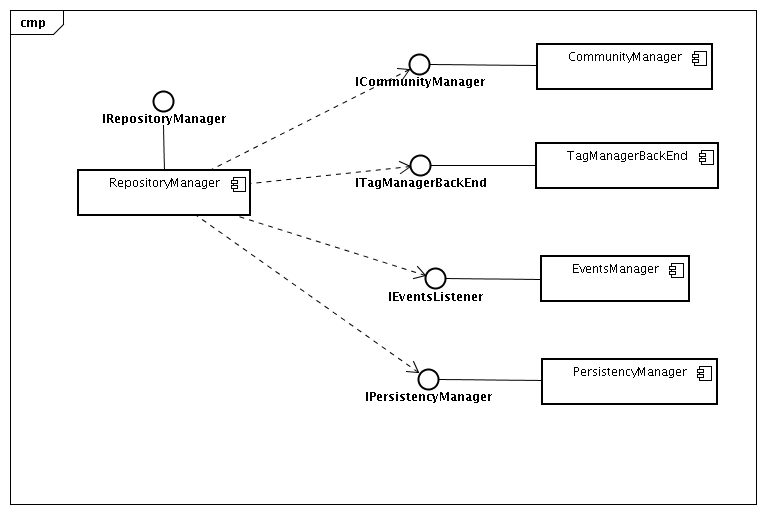
\includegraphics[scale=0.4]{diagrams/RepositoryManagerComponentsDiagram.png}
  \caption{\label{img:rm-components}RepositoryManager (components diagram)}
 \end{center}
\end{figure}

\subsubsection{Interface definition}

The next step carried on was defining an interface. The Tables
\ref{table:rm-interface-1}, \ref{table:rm-interface-2},
\ref{table:rm-interface-3} and \ref{table:rm-interface-4} summarize the
methods offered by the final version of \verb|RepositoryManager|.

%%tables with repository inteface
%%% Tables for repository interface %%%%
\begin{table}[h!]
	\small
    \begin{center}
		\begin{tabular}{||r|l|l||}
        
        %%%%%%%% Begin method %%%%%%%%%%%%%%%%%%
		\hline \hline
		\multicolumn{3}{||c||}{\bfseries{createSharedApplication}} \\
		\hline
		\hline 
		\multicolumn{3}{||l||}{Description: Create a new shared application in the
		repository.} \\
		\hline \hline
			Parameter & Type & Description \\
		\hline \hline
			appId & String & Application identifier in the standard ASTRA format. \\
			userId & String & Identifier of the user who uploads the application. \\
			appType & String & Type of application. \\
			appDescription & String & Application description. \\
		\hline \hline
		\multicolumn{3}{||l||}{Returns: Boolean, true if everything is ok, false if
		there was a failure.} \\
		\hline \hline
		%%%%%%%%%%%% End method %%%%%%%%%%%%%%%%%%%%%%
		
		%%%%%%%% Begin method %%%%%%%%%%%%%%%%%%
		\hline \hline
		\multicolumn{3}{||c||}{\bfseries{deleteSharedApplication}} \\
		\hline
		\hline 
		\multicolumn{3}{||l||}{Description: Delete a SharedApplication in the
		repository.} \\ \hline \hline
			Parameter & Type & Description \\
		\hline \hline
			appId & String & Application identifier in the standard ASTRA format \\
		\hline \hline
		\multicolumn{3}{||l||}{Returns: Boolean, true if the application was deleted
		properly, false otherwise.} \\
		\hline \hline
		%%%%%%%%%%%% End method %%%%%%%%%%%%%%%%%%%%%%
		
		%%%%%%%% Begin method %%%%%%%%%%%%%%%%%%
		\hline \hline
		\multicolumn{3}{||c||}{\bfseries{shareInCommunity}} \\
		\hline
		\hline 
		\multicolumn{3}{||l||}{Description: Store relationship between a shared 
		application and a community.} \\ \hline \hline
			Parameter & Type & Description \\
		\hline \hline
			userId & String & User identifier in the standard format. \\
			appId & String & Application identifier in the standard ASTRA format. \\
			communityId & String & Community identifier in the standard format. \\
		\hline \hline
		\multicolumn{3}{||l||}{Returns: Boolean, true if the operation was successful,
		false otherwise.} \\ \hline \hline
		%%%%%%%%%%%% End method %%%%%%%%%%%%%%%%%%%%%%
		
		%%%%%%%% Begin method %%%%%%%%%%%%%%%%%%
		\hline \hline
		\multicolumn{3}{||c||}{\bfseries{createSharedRule}} \\
		\hline
		\hline 
		\multicolumn{3}{||l||}{Description: Create a new shared rule associated to
		the application.} \\ \hline \hline Parameter & Type & Description \\
		\hline \hline
			userId & String & User identifier in the standard format. \\
			appId & String & Application identifier in the standard ASTRA format. \\
			ruleId & String & Rule identifier in the standard format. \\
			xmlData & String & XML file which contains the rule. \\
		\hline \hline
		\multicolumn{3}{||l||}{Returns: Boolean, true if the operation was successful,
		false otherwise.} \\ \hline \hline
		%%%%%%%%%%%% End method %%%%%%%%%%%%%%%%%%%%%%
		
		\end{tabular}
		\caption{\label{table:rm-interface-1} RepositoryManager interface}
	\end{center}
\end{table}


\begin{table}[h!]
	\small
    \begin{center}
		\begin{tabular}{||r|l|l||}

        %%%%%%%% Begin method %%%%%%%%%%%%%%%%%%
		\hline \hline
		\multicolumn{3}{||c||}{\bfseries{listSharedApplications}} \\
		\hline
		\hline 
		\multicolumn{3}{||l||}{Description: Returns the list of applications in the
		repository visible for that user.} \\ 
		\hline \hline 
		Parameter & Type & Description \\ 
		\hline \hline
			userId & String & User identifier in the standard format. \\
		\hline \hline
		\multicolumn{3}{||l||}{Returns: String array, list of applications.} \\
		\hline \hline
		%%%%%%%%%%%% End method %%%%%%%%%%%%%%%%%%%%%%
        
		%%%%%%%% Begin method %%%%%%%%%%%%%%%%%%
		\hline \hline
		\multicolumn{3}{||c||}{\bfseries{listSharedRules}} \\
		\hline
		\hline 
		\multicolumn{3}{||l||}{Description: Returns the list of rules in the
		repository associated to appID} \\ 
		\hline \hline 
		Parameter & Type & Description \\ 
		\hline \hline
			appId & String & Application identifier in the standard ASTRA format. \\
		\hline \hline
		\multicolumn{3}{||l||}{Returns: String array, list of rule identifiers.} \\
		\hline \hline
		%%%%%%%%%%%% End method %%%%%%%%%%%%%%%%%%%%%%
		
		%%%%%%%% Begin method %%%%%%%%%%%%%%%%%%
		\hline \hline
		\multicolumn{3}{||c||}{\bfseries{getXmlData}} \\
		\hline
		\hline 
		\multicolumn{3}{||l||}{Description: Returns the XML file which describes the
		rule.} \\ \hline \hline 
		Parameter & Type & Description \\ 
		\hline \hline
			appId & String & Application identifier in the standard ASTRA format. \\
			ruleId & String & Rule identifier in the standard format. \\
		\hline \hline
		\multicolumn{3}{||l||}{Returns: String, XML file describing the rule.} \\
		\hline \hline
		%%%%%%%%%%%% End method %%%%%%%%%%%%%%%%%%%%%%
		
		%%%%%%%% Begin method %%%%%%%%%%%%%%%%%%
		\hline \hline
		\multicolumn{3}{||c||}{\bfseries{getSharedApplicationName}} \\
		\hline
		\hline 
		\multicolumn{3}{||l||}{Description: Returns the name of the application.} \\
		\hline \hline Parameter & Type & Description \\ 
		\hline \hline
			appId & String & Application identifier in the standard ASTRA format. \\
		\hline \hline
		\multicolumn{3}{||l||}{Returns: String, application name.} \\
		\hline \hline
		%%%%%%%%%%%% End method %%%%%%%%%%%%%%%%%%%%%%
	
		%%%%%%%% Begin method %%%%%%%%%%%%%%%%%%
		\hline \hline
		\multicolumn{3}{||c||}{\bfseries{getSharedApplicationOwner}} \\
		\hline
		\hline 
		\multicolumn{3}{||l||}{Description: Returns the owner of the application.} \\
		\hline \hline Parameter & Type & Description \\ 
		\hline \hline
			appId & String & Application identifier in the standard ASTRA format. \\
		\hline \hline
		\multicolumn{3}{||l||}{Returns: String, application owner.} \\
		\hline \hline
		%%%%%%%%%%%% End method %%%%%%%%%%%%%%%%%%%%%%		
		
		%%%%%%%% Begin method %%%%%%%%%%%%%%%%%%
		\hline \hline
		\multicolumn{3}{||c||}{\bfseries{getSharedApplicationDescription}} \\
		\hline
		\hline 
		\multicolumn{3}{||l||}{Description: Returns the description of the
		application.} \\ \hline \hline Parameter & Type & Description \\ 
		\hline \hline
			appId & String & Application identifier in the standard ASTRA format. \\
		\hline \hline
		\multicolumn{3}{||l||}{Returns: String, application description.} \\
		\hline \hline
		%%%%%%%%%%%% End method %%%%%%%%%%%%%%%%%%%%%%		
		
		
		\end{tabular}
		\caption{\label{table:rm-interface-2} RepositoryManager interface (II)}
	\end{center}
\end{table}

\begin{table}[h!]
	\small
    \begin{center}
		\begin{tabular}{||r|l|l||}
        

        
        %%%%%%%% Begin method %%%%%%%%%%%%%%%%%%
		\hline \hline
		\multicolumn{3}{||c||}{\bfseries{getSharedApplicationDate}} \\
		\hline
		\hline 
		\multicolumn{3}{||l||}{Description: Returns the date of the
		application.} \\ \hline \hline Parameter & Type & Description \\ 
		\hline \hline
			appId & String & Application identifier in the standard ASTRA format. \\
		\hline \hline
		\multicolumn{3}{||l||}{Returns: String, application date.} \\
		\hline \hline
		%%%%%%%%%%%% End method %%%%%%%%%%%%%%%%%%%%%%			
        
	
		%%%%%%%% Begin method %%%%%%%%%%%%%%%%%%
		\hline \hline
		\multicolumn{3}{||c||}{\bfseries{getSharedApplicationType}} \\
		\hline
		\hline 
		\multicolumn{3}{||l||}{Description: Returns the type of the
		application.} \\ \hline \hline Parameter & Type & Description \\ 
		\hline \hline
			appId & String & Application identifier in the standard ASTRA format. \\
		\hline \hline
		\multicolumn{3}{||l||}{Returns: String, application type.} \\
		\hline \hline
		%%%%%%%%%%%% End method %%%%%%%%%%%%%%%%%%%%%%	
		
				%%%%%%%% Begin method %%%%%%%%%%%%%%%%%%
		\hline \hline
		\multicolumn{3}{||c||}{\bfseries{isAlreadyShared}} \\
		\hline
		\hline 
		\multicolumn{3}{||l||}{Description: Checks if an application has already been
		shared.} \\ \hline \hline Parameter & Type & Description \\ \hline \hline
			appId & String & Application identifier in the standard ASTRA format. \\
		\hline \hline
		\multicolumn{3}{||l||}{Returns: Boolean, true if already exists, false
		otherwise.} \\ \hline \hline
		%%%%%%%%%%%% End method %%%%%%%%%%%%%%%%%%%%%%	
		
		%%%%%%%% Begin method %%%%%%%%%%%%%%%%%%
		\hline \hline
		\multicolumn{3}{||c||}{\bfseries{getXmlRuleDescription}} \\
		\hline
		\hline 
		\multicolumn{3}{||l||}{Description: Returns a description of the rule in a
		readable} \\ 
		\multicolumn{3}{||l||}{way using the XML file information.} \\ 
		
		\hline \hline 
		Parameter & Type & Description \\ 
		\hline \hline
			appId & String & Application identifier in the standard ASTRA format. \\
			ruleId & String & Rule identifier in the standard format. \\
		\hline \hline
		\multicolumn{3}{||l||}{Returns: String, description of the rule.} \\
		\hline \hline
		%%%%%%%%%%%% End method %%%%%%%%%%%%%%%%%%%%%%
		
		%%%%%%%% Begin method %%%%%%%%%%%%%%%%%%
		\hline \hline
		\multicolumn{3}{||c||}{\bfseries{getXmlRule}} \\
		\hline
		\hline 
		\multicolumn{3}{||l||}{Description: Returns the XML file which describes the
		rule with} \\ 
		\multicolumn{3}{||l||}{the ownership already modified.} \\ 
		
		\hline \hline 
		Parameter & Type & Description \\ 
		\hline \hline
			appId & String & Application identifier in the standard ASTRA format. \\
			ruleId & String & Rule identifier in the standard format. \\
			newUserId & String & New user identifier in the standard format. \\
		\hline \hline
		\multicolumn{3}{||l||}{Returns: String, XML file associated to the rule.} \\
		\hline \hline
		%%%%%%%%%%%% End method %%%%%%%%%%%%%%%%%%%%%%
		

		

		
		\end{tabular}
		\caption{\label{table:rm-interface-3} RepositoryManager interface (III)}
	\end{center}
\end{table}

% \begin{table}[h!]
% 	\small
%     \begin{center}
% 		\begin{tabular}{||r|l|l||}
% 		
% 
% 	
% 		\end{tabular}
% 		\caption{\label{table:rm-interface-4} Repository Manager interface (IV)}
% 	\end{center}
% \end{table}


\begin{table}[h!]
	\small
    \begin{center}
		\begin{tabular}{||r|l|l||}
		
				%%%%%%%% Begin method %%%%%%%%%%%%%%%%%%
		\hline \hline
		\multicolumn{3}{||c||}{\bfseries{search (overloaded)}} \\
		\hline
		\hline 
		\multicolumn{3}{||l||}{Description: It performs a search according to one
		criterion.} \\ \hline \hline Parameter & Type & Description \\ 
		\hline \hline
			userId & String & Identifier of the user who is performing the search.\\
			q & String & Query. \\
			criterion & String & Criterion to use. \\
		\hline \hline
		\multicolumn{3}{||l||}{Returns: String array, with the identifiers of the
		matching applications.} \\ \hline \hline
		%%%%%%%%%%%% End method %%%%%%%%%%%%%%%%%%%%%%
	
		%%%%%%%% Begin method %%%%%%%%%%%%%%%%%%
		\hline \hline
		\multicolumn{3}{||c||}{\bfseries{search (overloaded)}} \\
		\hline
		\hline 
		\multicolumn{3}{||l||}{Description: It performs a search according to a set
		of criteria.} \\ \hline \hline Parameter & Type & Description \\ 
		\hline \hline
			userId & String & Identifier of the user who is performing the search.\\
			q & String & Query. \\
			criteria & String array & Criteria to use. \\
		\hline \hline
		\multicolumn{3}{||l||}{Returns: String array, with the identifiers of the
		matching applications.} \\ \hline \hline
		%%%%%%%%%%%% End method %%%%%%%%%%%%%%%%%%%%%%
		
		%%%TO-DO: THIS ONE MAY CHANGE AFTER THE TESTS!!!
		%%%%%%%% Begin method %%%%%%%%%%%%%%%%%%
		\hline \hline
		\multicolumn{3}{||c||}{\bfseries{searchBySimilarity}} \\
		\hline
		\hline 
		\multicolumn{3}{||l||}{Description: It performs a search of similar
		applications.} \\ \hline \hline Parameter & Type & Description \\ \hline
		\hline userId & String & Identifier of the user who is performing the
		search.\\ 
		appId & String & Application identifier in the standard ASTRA format. \\
			appDescription & String & Application description. \\
		\hline \hline
		\multicolumn{3}{||l||}{Returns: String array, with the identifiers of the
		matching applications.} \\ \hline \hline
		%%%%%%%%%%%% End method %%%%%%%%%%%%%%%%%%%%%%
		
		\end{tabular}
		\caption{\label{table:rm-interface-4} RepositoryManager interface (IV)}
	\end{center}
\end{table}

\clearpage


\subsubsection{Classes definition}
\label{subsec:rm-classes-definition}

The functionalities of this bundle are structured in a set of classes from
which we will remark:

\begin{itemize}
  \item \verb|RepositoryManagerImpl|:
	\begin{itemize}
      \item It implements all the methods of \verb|IRepositoryManager|. 
      \item It manages the connection with the rest of the bundles.
      \item It takes care of the integration with the search engine. 
    \end{itemize}
  \item \verb|SharedApplication|: It represents an application in the
  repository. It is composed by \verb|SharedRules|.
  \item \verb|SharedRule|: It represents a shared rule in the repository.
  \item \verb|SearchEngine|: It implements a search engine to perform queries
  about the applications in the repository.
   \item \verb|XMLFunctionalities|: Class which provides auxiliar abstract
   methods related to the XML functionalities (i.e. method to create a rule
   description receiving the XML file).
\end{itemize}

The Figure \ref{img:rm-cd} shows the most important classes with its main
methods, and the relationship between them. \newline


\begin{figure}[h!]
 \begin{center}
 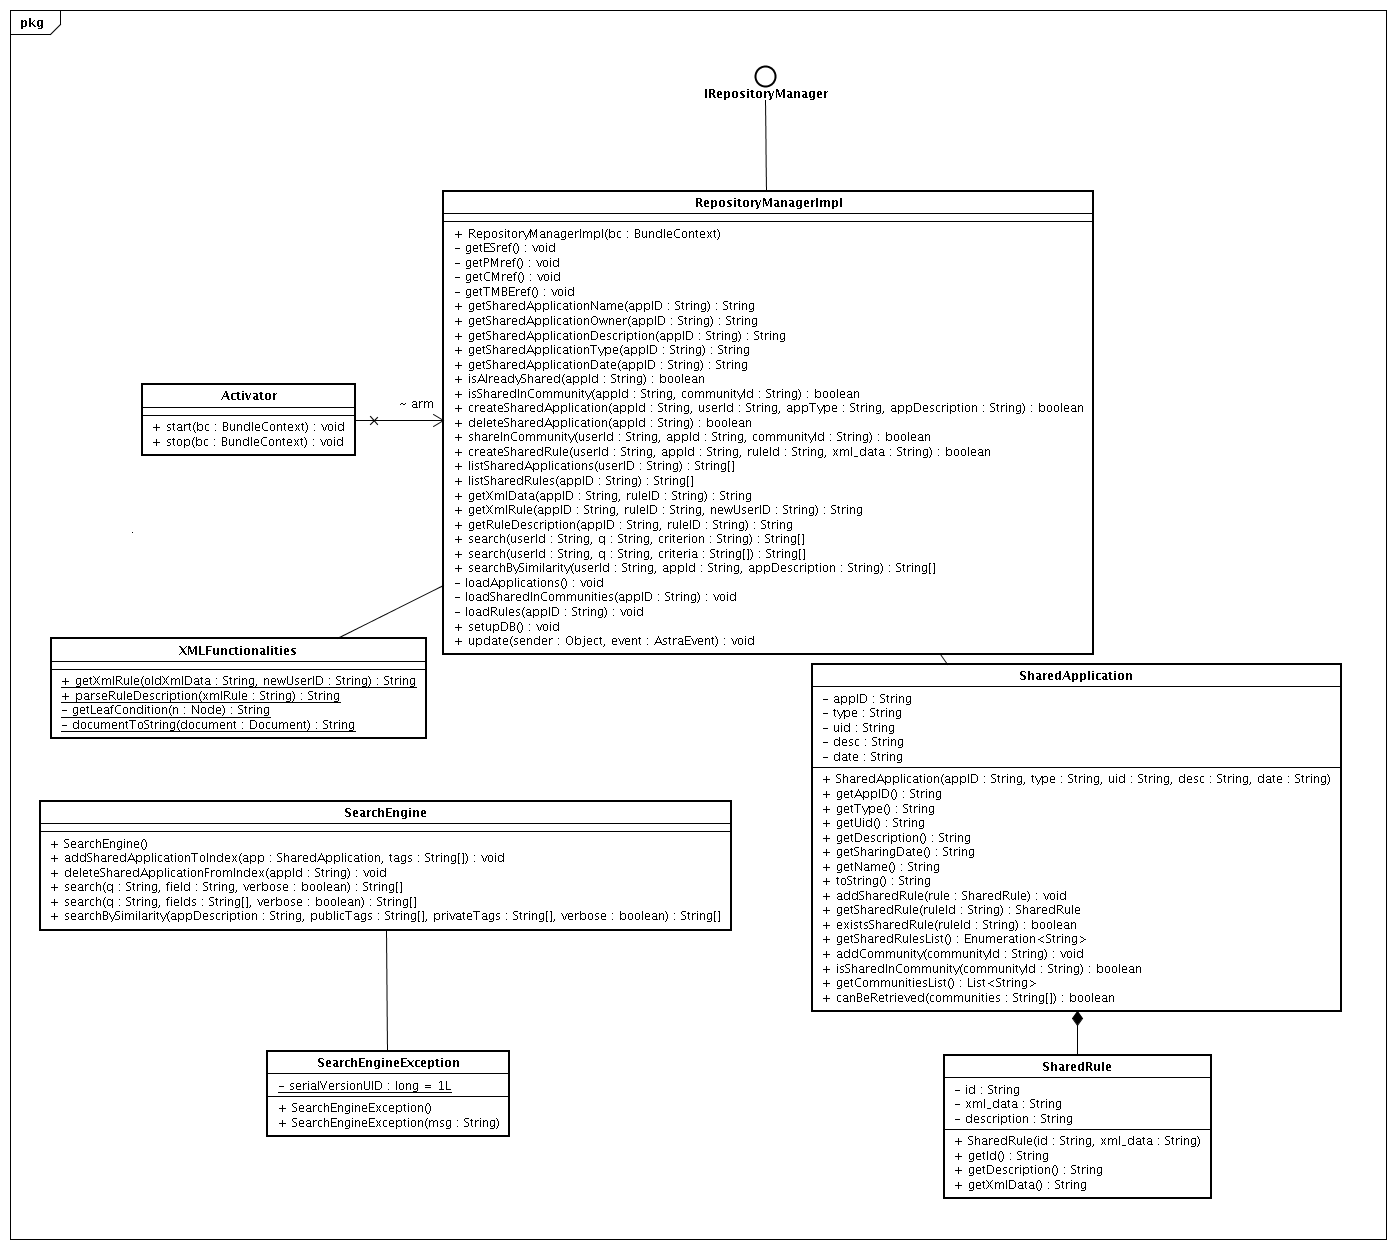
\includegraphics[scale=0.31]{diagrams/RepositoryManagerClassDiagram.png}
  \caption{\label{img:rm-cd}RepositoryManager (class diagram)}
 \end{center}
\end{figure}

\subsubsection{Storage system}

Finally, we needed to design a database model for \verb|RepositoryManager|. We
designed it taking into account the following relationships:

\begin{itemize}
  \item An user owns (has shared) \verb|0..n| applications in the repository.
  \item A shared application has \verb|1..n| shared rules.
  \item A shared application is visible for \verb|1..n| communities.
  \item A community has \verb|0..n| shared applications.
  \item A shared application has \verb|0..n| tags.
\end{itemize}

The Figure \ref{img:rm-db-model} shows a database diagram with all the
necessary tables and the relationships between them which were previously
enumerated.


\begin{figure}[h!]
 \begin{center}
 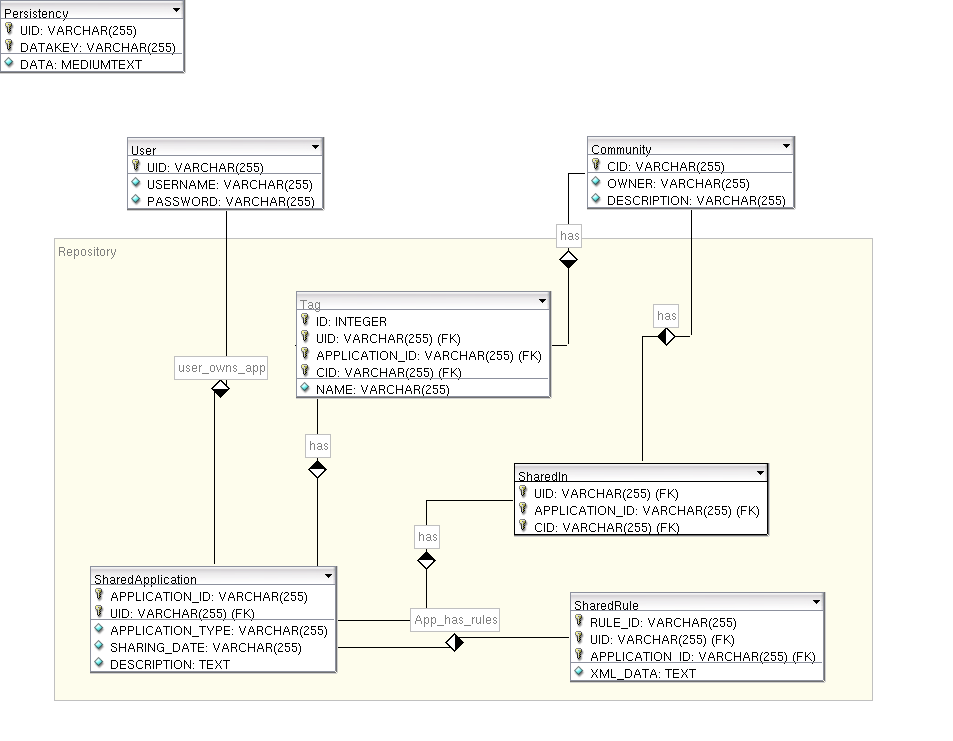
\includegraphics[scale=0.4]{diagrams/RepositoryManagerDBModel.png}
  \caption{\label{img:rm-db-model}RepositoryManager (database model)}
 \end{center}
\end{figure}

It is also important to remark that in order to increase the performance in
querying, the repository keeps also a copy in memory of all the
information about the applications and the rules stored. This
information is stored in hash tables that are synchronized with the data in the
database.
\newline
This decision introduces as a drawback the need of duplicating the number of
create and delete operations (which have to be executed in memory and in the
database) and arises the need of establishing synchronization mechanisms to have
consistent copies in both sides. But considering that most of the operations are
to retrieve information (i.e.: all the needed operations for searching or
getting an application) the global performance also increases.


%%%%%%%%%%%%%%% TagManagerBackEnd %%%%%%%%%%%%%%%%%%%%%%%%%

\subsection{TagManagerBackEnd}
\label{subsec:tmbe-design}

As it was explained in Section \ref{subsec:bundles-design} we decided to divide
the tags management into two components: \verb|TagManagerBackEnd| and
\verb|TagManagerNode| (which will be explained in Section
\ref{subsec:tmn-design}).
\newline
\verb|TagManagerBackEnd| is the bundle that manages the public and community
tags. It is executed in the Backend, and it possess an interface to make its
services available to the rest of the bundles in ASTRA. 
The initial version of the code was based on the code for a tagging system under
the project Ubicollab\footnote{Ubiquitous Collaboration: is an open source
project aiming at implementing a platform for mobile communities developed at
NTNU (http://ubicollab.idi.ntnu.no).} by Christian Laverton, which is licensed
under an Apache License (version 2.0). It was first adapted for ASTRA, and 
extended afterwards.
\newline
In this section we will explain the process we followed to carry on its design, 
taking a similar approach to the one we took to design \verb|RepositoryManager|
(Section \ref{subsec:repository-design}).


\subsubsection{Connection with other bundles}
\label{subsubsec:connections-tmbe}

The first step consisted of defining the relationship between
\verb|TagManagerBackEnd| and the rest of the bundles in ASTRA.

Taking into account the requirements stated in Section \ref{sec:requirements}
and the analysis performed in Section \ref{subsec:tags-use-cases}, we needed to
make use of the services of the following bundles:

\begin{itemize}
  \item \verb|CommunityManager|: Necessary to retrieve information about the
  relationship between users, their communities and the tags. I.e.: to
  make available certain tag taking into account the scope in terms of 
  visibility of the user.
  \item \verb|EventsManager|: Necessary to give feedback of the events produced
  in it. I.e: to inform other bundles that a tag has been added.
  \item \verb|PersistencyManager|: Necessary to store permanently all the data
  into the database. Using its services, we assure the robustness of the system.
\end{itemize}

The Figure \ref{img:tmbe-components} shows graphically the relationship between
\verb|TagManagerBackEnd| and the rest of components through its interfaces.

\begin{figure}[h!]
 \begin{center}
 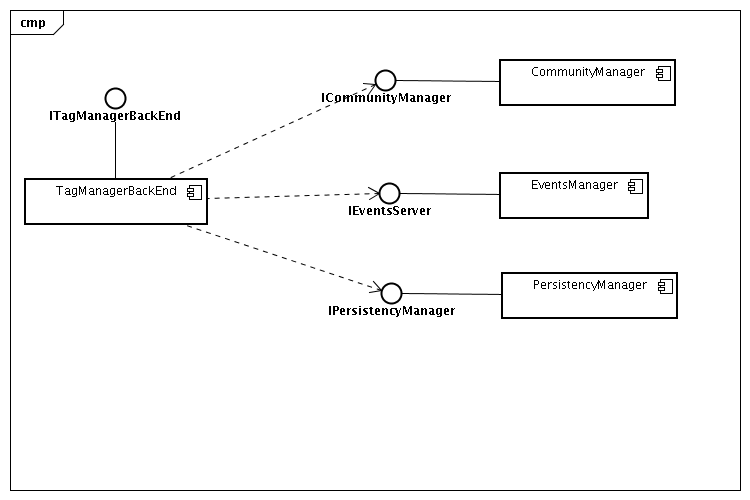
\includegraphics[scale=0.4]{diagrams/TagManagerBackEndComponentsDiagram.png}
  \caption{\label{img:tmbe-components}TagManagerBackEnd (components diagram)}
 \end{center}
\end{figure}

\subsubsection{Interface definition}
\label{subsubsec:tmbe-interface-definition}

The next step consisted of defining its interface. The Tables
\ref{table:tmbe-interface-1} and \ref{table:tmbe-interface-2} summarize the
methods offered by the final version of \verb|TagManagerBackEnd|.

%%tables with repository inteface
%%% Tables for tmbe interface %%%%
\begin{table}[h!]
	\small
    \begin{center}
		\begin{tabular}{||r|l|l||}
        
        %%%%%%%% Begin method %%%%%%%%%%%%%%%%%%
		\hline \hline
		\multicolumn{3}{||c||}{\bfseries{addTag (overloaded)}} \\
		\hline
		\hline 
		\multicolumn{3}{||l||}{Description: Creates a public tag.} \\
		\hline \hline
			Parameter & Type & Description \\
		\hline \hline
			name & String & Tag name. \\
			appId & String & Application identifier in the standard ASTRA format. \\
			userId & String & Identifier of the user who tags the application. \\
		\hline \hline
		\multicolumn{3}{||l||}{Returns: Boolean, true if the operation was successful,
		false otherwise.} \\ \hline \hline
		%%%%%%%%%%%% End method %%%%%%%%%%%%%%%%%%%%%%
		
		%%%%%%%% Begin method %%%%%%%%%%%%%%%%%%
		\hline \hline
		\multicolumn{3}{||c||}{\bfseries{addTag (overloaded)}} \\
		\hline
		\hline 
		\multicolumn{3}{||l||}{Description: Creates a tag only visible for that
		community.} \\ \hline \hline
			Parameter & Type & Description \\
		\hline \hline
			name & String & Tag name. \\
			appId & String & Application identifier in the standard ASTRA format. \\
			userId & String & Identifier of the user who tags the application. \\
			communityId & String & Community identifier. \\
		\hline \hline
		\multicolumn{3}{||l||}{Returns: Boolean, true if the operation was successful,
		false otherwise.} \\ \hline \hline
		%%%%%%%%%%%% End method %%%%%%%%%%%%%%%%%%%%%%


		%%%%%%%% Begin method %%%%%%%%%%%%%%%%%%
		\hline \hline
		\multicolumn{3}{||c||}{\bfseries{getTags}} \\
		\hline
		\hline 
		\multicolumn{3}{||l||}{Description: Returns a list of public tags for the
		given application.} \\ 
		\hline \hline 
			Parameter & Type & Description \\
		\hline \hline
			appId & String & Application identifier in the standard ASTRA format. \\
			limit & Integer & Limit on number of results returned. \\ \hline \hline
		\multicolumn{3}{||l||}{Returns: String array, list of public tags for the
		given application.} \\
		\hline
		\hline
		%%%%%%%%%%%% End method %%%%%%%%%%%%%%%%%%%%%%	
		
		
				%%%%%%%% Begin method %%%%%%%%%%%%%%%%%%
		\hline \hline
		\multicolumn{3}{||c||}{\bfseries{getTagsByCommunity}} \\
		\hline
		\hline 
		\multicolumn{3}{||l||}{Description: Returns a list of public tags for the
		given application and community.} \\ 
		\hline \hline 
			Parameter & Type & Description \\
		\hline \hline
			appId & String & Application identifier in the standard ASTRA format. \\
			limit & Integer & Limit on number of results returned. \\
			communityId & String & Community identifier. \\
		\hline \hline
		\multicolumn{3}{||l||}{Returns: String array, list of public tags for the
		given application and community.} \\
		\hline
		\hline
		%%%%%%%%%%%% End method %%%%%%%%%%%%%%%%%%%%%%	
		
		\end{tabular}
		\caption{\label{table:tmbe-interface-1} TagManagerBackEnd interface}
	\end{center}
\end{table}

\begin{table}[h!]
	\small
    \begin{center}
		\begin{tabular}{||r|l|l||}
        
       
		%%%%%%%% Begin method %%%%%%%%%%%%%%%%%%
		\hline \hline
		\multicolumn{3}{||c||}{\bfseries{getTagsByApplication}} \\
		\hline
		\hline 
		\multicolumn{3}{||l||}{Description: Returns a list of tags associated to 
		the application	which are public} \\ 
		\multicolumn{3}{||l||}{or visible for that user (because he belongs to
		that community).} \\ \hline \hline 
			Parameter & Type & Description \\
		\hline \hline
			appId & String & Application identifier in the standard ASTRA format. \\
			userId & String & User identifier. \\
			limit & Integer & Limit on number of results returned. \\
		\hline \hline
		\multicolumn{3}{||l||}{Returns: String array, list of visible tags for this
		user associated to the given application.}
		\\
		\hline
		\hline
		%%%%%%%%%%%% End method %%%%%%%%%%%%%%%%%%%%%%	
		
		
				%%%%%%%% Begin method %%%%%%%%%%%%%%%%%%
		\hline \hline
		\multicolumn{3}{||c||}{\bfseries{deleteTag (overloaded)}} \\
		\hline
		\hline 
		\multicolumn{3}{||l||}{Description: Deletes a public tag.} \\
		\hline \hline
			Parameter & Type & Description \\
		\hline \hline
			name & String & Tag name. \\
			appId & String & Application identifier in the standard ASTRA format. \\
			userId & String & Identifier of the user who tagged the application. \\
		\hline \hline
		\multicolumn{3}{||l||}{Returns: Boolean, true if the operation was successful,
		false otherwise.} \\ \hline \hline
		%%%%%%%%%%%% End method %%%%%%%%%%%%%%%%%%%%%%
		
		%%%%%%%% Begin method %%%%%%%%%%%%%%%%%%
		\hline \hline
		\multicolumn{3}{||c||}{\bfseries{deleteTag (overloaded)}} \\
		\hline
		\hline 
		\multicolumn{3}{||l||}{Description: Deletes a tag for a given community.} \\
		\hline \hline
			Parameter & Type & Description \\
		\hline \hline
			name & String & Tag name. \\
			appId & String & Application identifier in the standard ASTRA format. \\
			userId & String & Identifier of the user who tagged the application. \\
			communityId & String & Community identifier. \\
		\hline \hline
		\multicolumn{3}{||l||}{Returns: Boolean, true if the operation was successful,
		false otherwise.} \\ \hline \hline
		%%%%%%%%%%%% End method %%%%%%%%%%%%%%%%%%%%%%
		
	
		\end{tabular}
		\caption{\label{table:tmbe-interface-2} TagManagerBackEnd interface (II)}
	\end{center}
\end{table}


% 
% \begin{table}[h!]
% 	\small
%     \begin{center}
% 		\begin{tabular}{||r|l|l||}
%         
% 
% 		
% 		\end{tabular}
% 		\caption{\label{table:tmbe-interface-3} Tag Manager Backend interface (III)}
% 	\end{center}
% \end{table}


\clearpage

\subsubsection{Classes definition}
The definition of the classes in this case is simpler than the one explained in
Section \ref{subsec:rm-classes-definition}: the main functionalities are
provided by the class \verb|TagManagerBackEnd|, which implements the methods of
the interface \verb|ITagManagerBackEnd| explained before in
Section \ref{subsubsec:tmbe-interface-definition} and is responsible for the
communication with the bundles.
\newline
The Figure \ref{img:tmbe-cd} shows the class diagram for this bundle.

\begin{figure}[h!]
 \begin{center}
 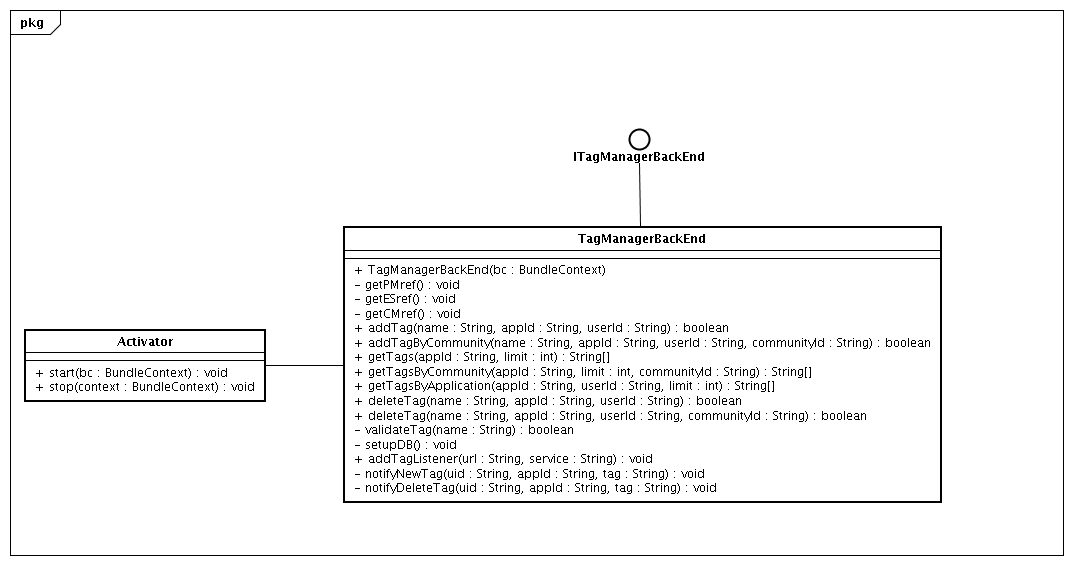
\includegraphics[scale=0.4]{diagrams/TagManagerBackEndClassDiagram.png}
  \caption{\label{img:tmbe-cd}TagManagerBackEnd (class diagram)}
 \end{center}
\end{figure}

\subsubsection{Storage system}
\label{subsubsec:tmbe-storage-system}
The storage system in this case is also simpler: it consists only of one
table as in the code in which was based, allowing back compatibility. 
\newline
The relationships between this table and the repository tables are shown in the
previously explained Figure \ref{img:rm-db-model}.

%%%%%%%%%%%%%%% TagManagerNode %%%%%%%%%%%%%%%%%%%%%%%%%
%\clearpage

\subsection{TagManagerNode}
\label{subsec:tmn-design}

As it was introduced in Section \ref{subsec:tmbe-design}, \verb|TagManagerNode|
is the bundle responsible for the private tags. It is executed in the nodes 
(client side), and it has an interface to offer its services to the rest of 
the bundles in ASTRA.
\newline

In this section we will explain the process we followed to carry on its design, 
taking a similar approach to the one we took previously. \verb|TagManagerNode|
is similar to \verb|TagManagerBackEnd| and, since it has to take care only of
private tags, its design is simpler. Therefore the explanation in this case
will not be so detailed and the reader will be forwarded to previous
subsections when a similar concept arises.

\subsubsection{Connection with other bundles}
\label{subsubsec:connections-tmn}
As is shown in Figure \ref{img:tmn-components}, \verb|TagManagerNode| needs only
the services of \verb|PersistencyManager|, which allow it to store its data
permanently.

\begin{figure}[h!]
 \begin{center}
 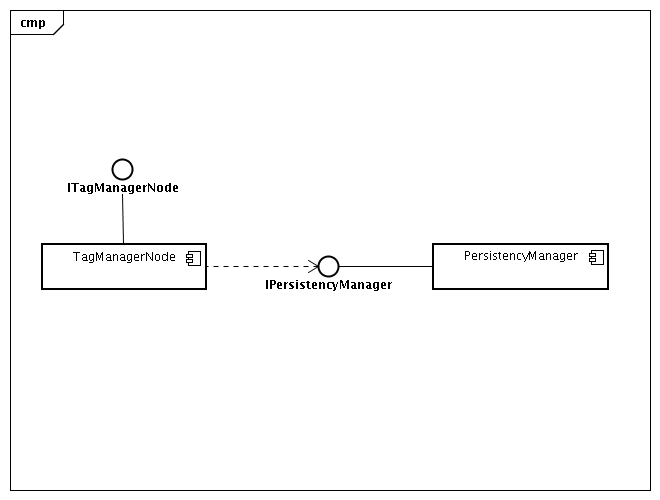
\includegraphics[scale=0.4]{diagrams/TagManagerNodeComponentsDiagram.png}
  \caption{\label{img:tmn-components}TagManagerNode (components diagram)}
 \end{center}
\end{figure}

\subsubsection{Interface definition}
\label{subsubsec:tmn-interface-definition}

\verb|TagManagerNode|`s interface is summarize in Table
\ref{table:tmn-interface}.

%%tables with repository inteface
%%% Tables for tmbe interface %%%%
\begin{table}[h!]
	\small
    \begin{center}
		\begin{tabular}{||r|l|l||}
        
        %%%%%%%% Begin method %%%%%%%%%%%%%%%%%%
		\hline \hline
		\multicolumn{3}{||c||}{\bfseries{addTag}} \\
		\hline
		\hline 
		\multicolumn{3}{||l||}{Description: Creates a new private tag.} \\
		\hline \hline
			Parameter & Type & Description \\
		\hline \hline
			name & String & Tag name. \\
			appId & String & Application identifier in the standard ASTRA format. \\
			userId & String & Identifier of the user who tags the application. \\
		\hline \hline
		\multicolumn{3}{||l||}{Returns: Boolean, true if the operation was successful,
		false otherwise.} \\ \hline \hline
		%%%%%%%%%%%% End method %%%%%%%%%%%%%%%%%%%%%%


		%%%%%%%% Begin method %%%%%%%%%%%%%%%%%%
		\hline \hline
		\multicolumn{3}{||c||}{\bfseries{getTags}} \\
		\hline
		\hline 
		\multicolumn{3}{||l||}{Description: Returns a list of private tags for the
		given application.} \\ 
		\hline \hline 
			Parameter & Type & Description \\
		\hline \hline
			appId & String & Application identifier in the standard ASTRA format. \\
			userId & String & Identifier of the user. \\
			limit & Integer & Limit on number of results returned. \\
		\hline \hline
		\multicolumn{3}{||l||}{Returns: String array, list of private tags for the
		given application.} \\
		\hline
		\hline
		%%%%%%%%%%%% End method %%%%%%%%%%%%%%%%%%%%%%	
		
		%%%%%%%% Begin method %%%%%%%%%%%%%%%%%%
		\hline \hline
		\multicolumn{3}{||c||}{\bfseries{deleteTag}} \\
		\hline
		\hline 
		\multicolumn{3}{||l||}{Description: Deletes a private tag.} \\
		\hline \hline
			Parameter & Type & Description \\
		\hline \hline
			name & String & Tag name. \\
			appId & String & Application identifier in the standard ASTRA format. \\
			userId & String & Identifier of the user who tagged the application. \\
		\hline \hline
		\multicolumn{3}{||l||}{Returns: Boolean, true if the operation was successful,
		false otherwise.} \\ \hline \hline
		%%%%%%%%%%%% End method %%%%%%%%%%%%%%%%%%%%%%

		
		\end{tabular}
		\caption{\label{table:tmn-interface} TagManagerNode interface}
	\end{center}
\end{table}


\clearpage

\subsubsection{Classes definition}
The main functionalities are provided by the class \verb|TagManagerNode| as is
shown in the Figure \ref{img:tmn-cd}.

\begin{figure}[h!]
 \begin{center}
 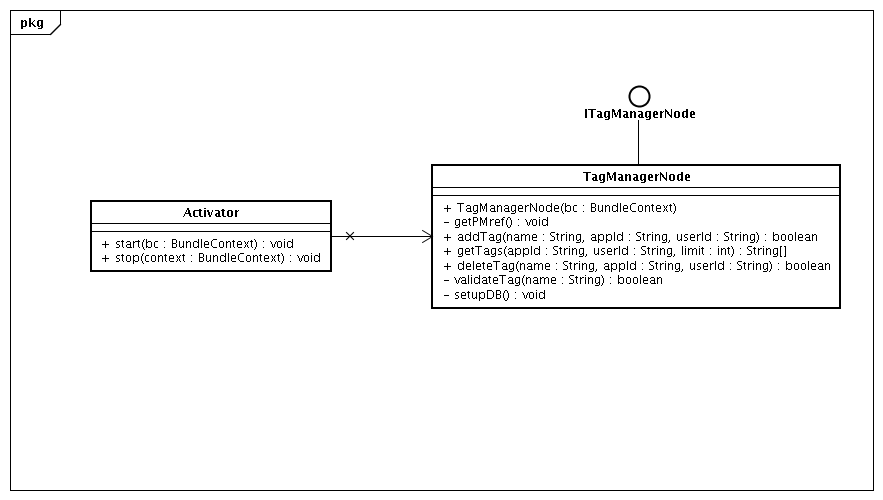
\includegraphics[scale=0.4]{diagrams/TagManagerNodeClassDiagram.png}
  \caption{\label{img:tmn-cd}TagManagerNode (class diagram)}
 \end{center}
\end{figure}

\subsubsection{Storage system}
It consists only of one table, following an schema similar to the one
explained in Section \ref{subsubsec:tmbe-storage-system}.

%%%%%%%%%%%%%%% ApplicationManager %%%%%%%%%%%%%%%%%%%%%%%%%
%\clearpage

\subsection{ApplicationManager}
\label{subsec:am-design}

The last bundle is \verb|ApplicationManager|, which is in charge of the
interaction with the user by offering an intuitive GUI, and the connection with
other ASTRA bundles services based on that interaction. It is executed in the
Node side, and it makes uses of the services offered by the bundles in both
edges: Node (client side) and Backend (server side).
\newline

In this section we will explain the process we followed to carry on its design.
The most important implementation details about this bundle are explained
in Section \ref{sec:implementation}.

\subsubsection{Connection with other bundles}
\label{subsubsec:connections-am}
First we need to analyze the relationship between this bundle and
the rest of bundles in ASTRA.
Taking into account the requirements stated in Section \ref{sec:requirements}
and the analysis performed in Section \ref{sec:use-cases}, it was necessary to
use the services of the following bundles:

\begin{itemize}
  \item Local bundles:
	\begin{itemize}
	  \item \verb|AwarenessApplicationManager|: Necessary to send and receive
	  information about the local applications.
	  \item \verb|AwarenessManager|: Necessary to send and receive information
	  about the local rules.
	  \item \verb|TagManagerNode|: Necessary to manage the private tags.
	  \item \verb|OntologyManager|: Necessary to assist the user in the application
	  adaptation process using ontologies\footnote{This feature is not available
	  in the current version of ASTRA, but \texttt{ApplicationManager} has been
	  prepared to be easily extended. A detailed explanation can be found in Section
	  \ref{subsec:implementation-app-adaptation}.}.
    \end{itemize}
   
   \item Remote bundles:
	\begin{itemize}
	  \item \verb|UserManager|: Necessary to authenticate the users during the
	  logging in process.
	  \item \verb|CommunityManager|: Necessary to retrieve information about the
	  communities joined by the user.
	  \item \verb|TagManagerBackend|: Necessary to manage the public and community
	  tags.
	  \item \verb|RepositoryManager|: Necessary to share and retrieve applications
	  with the rest of the users.
    \end{itemize}
    
\end{itemize}

The Figure \ref{img:am-components} shows graphically the relationship between
\verb|ApplicationManager| and the rest of bundles.

\begin{figure}[h!]
 \begin{center}
 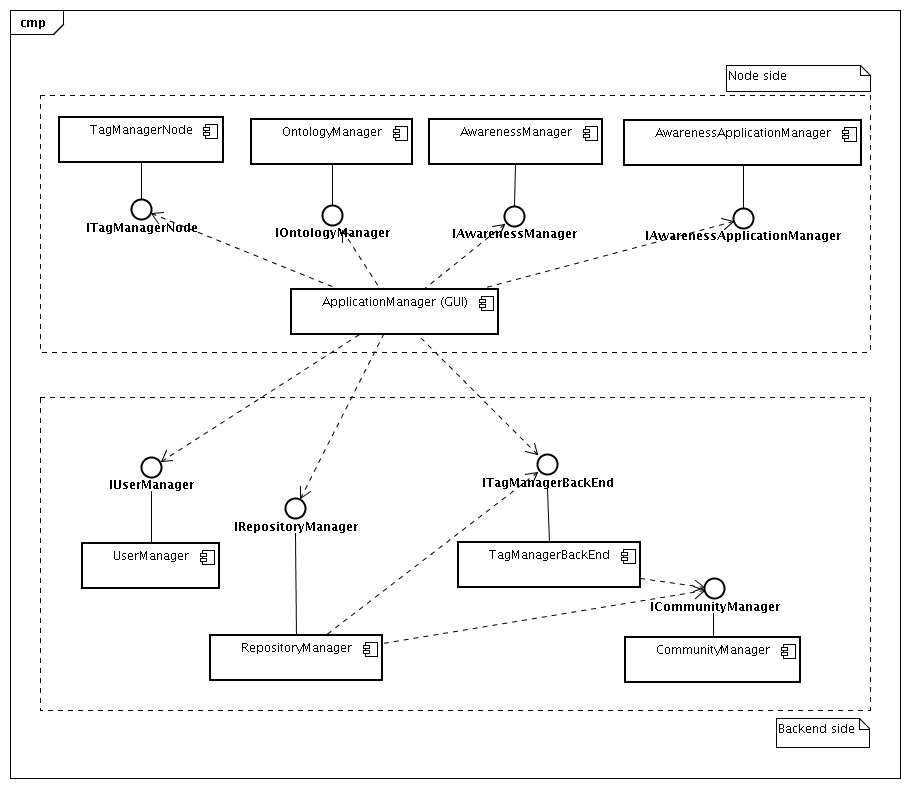
\includegraphics[scale=0.4]{diagrams/ApplicationManagerComponentsDiagram.png}
  \caption{\label{img:am-components}ApplicationManager (components diagram)}
 \end{center}
\end{figure}

\subsubsection{Bundle architecture}
\label{subsub:am-bundle-arch}
In this subsection we will explain briefly the architectural and design
patterns which are implemented by this bundle\footnote{The implementation
details will be stated in Section \ref{sec:implementation}.}, and we will
discuss the reasons why they were chosen.

%%\subsubsubsection{Singleton (design pattern)}

\paragraph{}

\textbf{Singleton (design pattern):}\newline

A design pattern is a description for a commonly recurring structure of communicating
components that solves a general design problem within a
particular context. It provides a scheme for refining the 
components of a software system and the relationships between them.
\newline
In order to implement the MVC architectural pattern, we made use of the
singleton design pattern in the controller. The singleton pattern makes the
class itself responsible for keeping track of its sole instance, ensuring that
no other instance can be created.
\newline
The Figure \ref{img:singleton} shows a singleton general class diagram.


\begin{figure}[h!]
 \begin{center}
 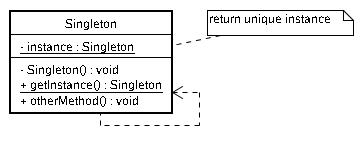
\includegraphics[scale=0.7]{img/singleton.jpg}
  \caption{\label{img:singleton}Singleton design pattern}
 \end{center}
\end{figure}

\paragraph{}

\textbf{MVC (architectural pattern):}\newline

An architectural pattern expresses a fundamental structural organisation or
schema for software systems. It provides a set of predefined subsystems,
specifies their responsibilities, and includes rules and
guidelines for organising the relationships between them.
\newline
\verb|ApplicationManager| implements a MVC (Model-View-Controller) pattern,
which allows us to isolate the business logic from the user interface, permitting one
to be freely modified without affecting the other. The controller collects
user input, the model manipulates application data, and the view presents
results to the user.
\newline
The details about how MVC was implemented in the bundle can be found in Section
\ref{sec:implementation}, and the design of the classes is explained in
Section \ref{subsub:am-classes-definition}.


\subsubsection{Classes definition}
\label{subsub:am-classes-definition}
As we stated in Section \ref{subsub:am-bundle-arch}, \verb|ApplicationManager|
implements a MVC pattern. Therefore the class definition is based on the structural
organization defined for this pattern which we can summarize as follows:

\begin{itemize}
	\item Controller: It is represented by the class
 	 \verb|ApplicationManagerController|, whose job is to contain the interactions
 	 of the user interface components and to interact with other ``business logic''
  	classes. It implements a singleton design pattern.
  	It needs basically to perform two functions:
	\begin{itemize}
  		\item To keep track of the references to the user interface components.
  		\item To provide a set of methods that other components can directly call in
  		their event handler.
    \end{itemize}
    
 	\item Model: It is represented by the class \verb|ApplicationManagerModel|,
 	which contains the ``business logic''. Taking into account the bundle nature
 	of\\ \verb|ApplicationManager|, the ``business logic'' in this case is
 	simpler, summarizing its functions in: 
	\begin{itemize}
  		\item To manage the references to the rest of the bundles.
  		\item To work as an ``stub container'' to make use of the services provided
  		by those.
  		\item To take care of the session data, i.e.: the user identifier.
    \end{itemize}
    Considering we are only go to need a single instance of the model, it also
    implements a singleton pattern\footnote{This is an specific decission for 
   this bundle, and it is not established by the MVC architectural pattern,
   actually in most of the cases the model does not implement it. }.
    
    \item View: It is represented by several classes whose task consist of
    presenting the information to the user. This includes all the classes which
    represent the windows (i.e.: \verb|MainWindow|, \verb|LoginWindow|, etc.)
    and all the necessary classes that extend some of the graphical components (i.e.:
    \verb|TreeRenderer|, \verb|TagListCellRenderer|, etc.)\footnote{These
    classes are ommited in Figure \ref{img:am-cd} in order to make it simpler.}.
\end{itemize}

The Figure \ref{img:am-cd} shows the most important classes that made up this
bundle and the relationships between them.

\begin{figure}[h!]
 \begin{center}
 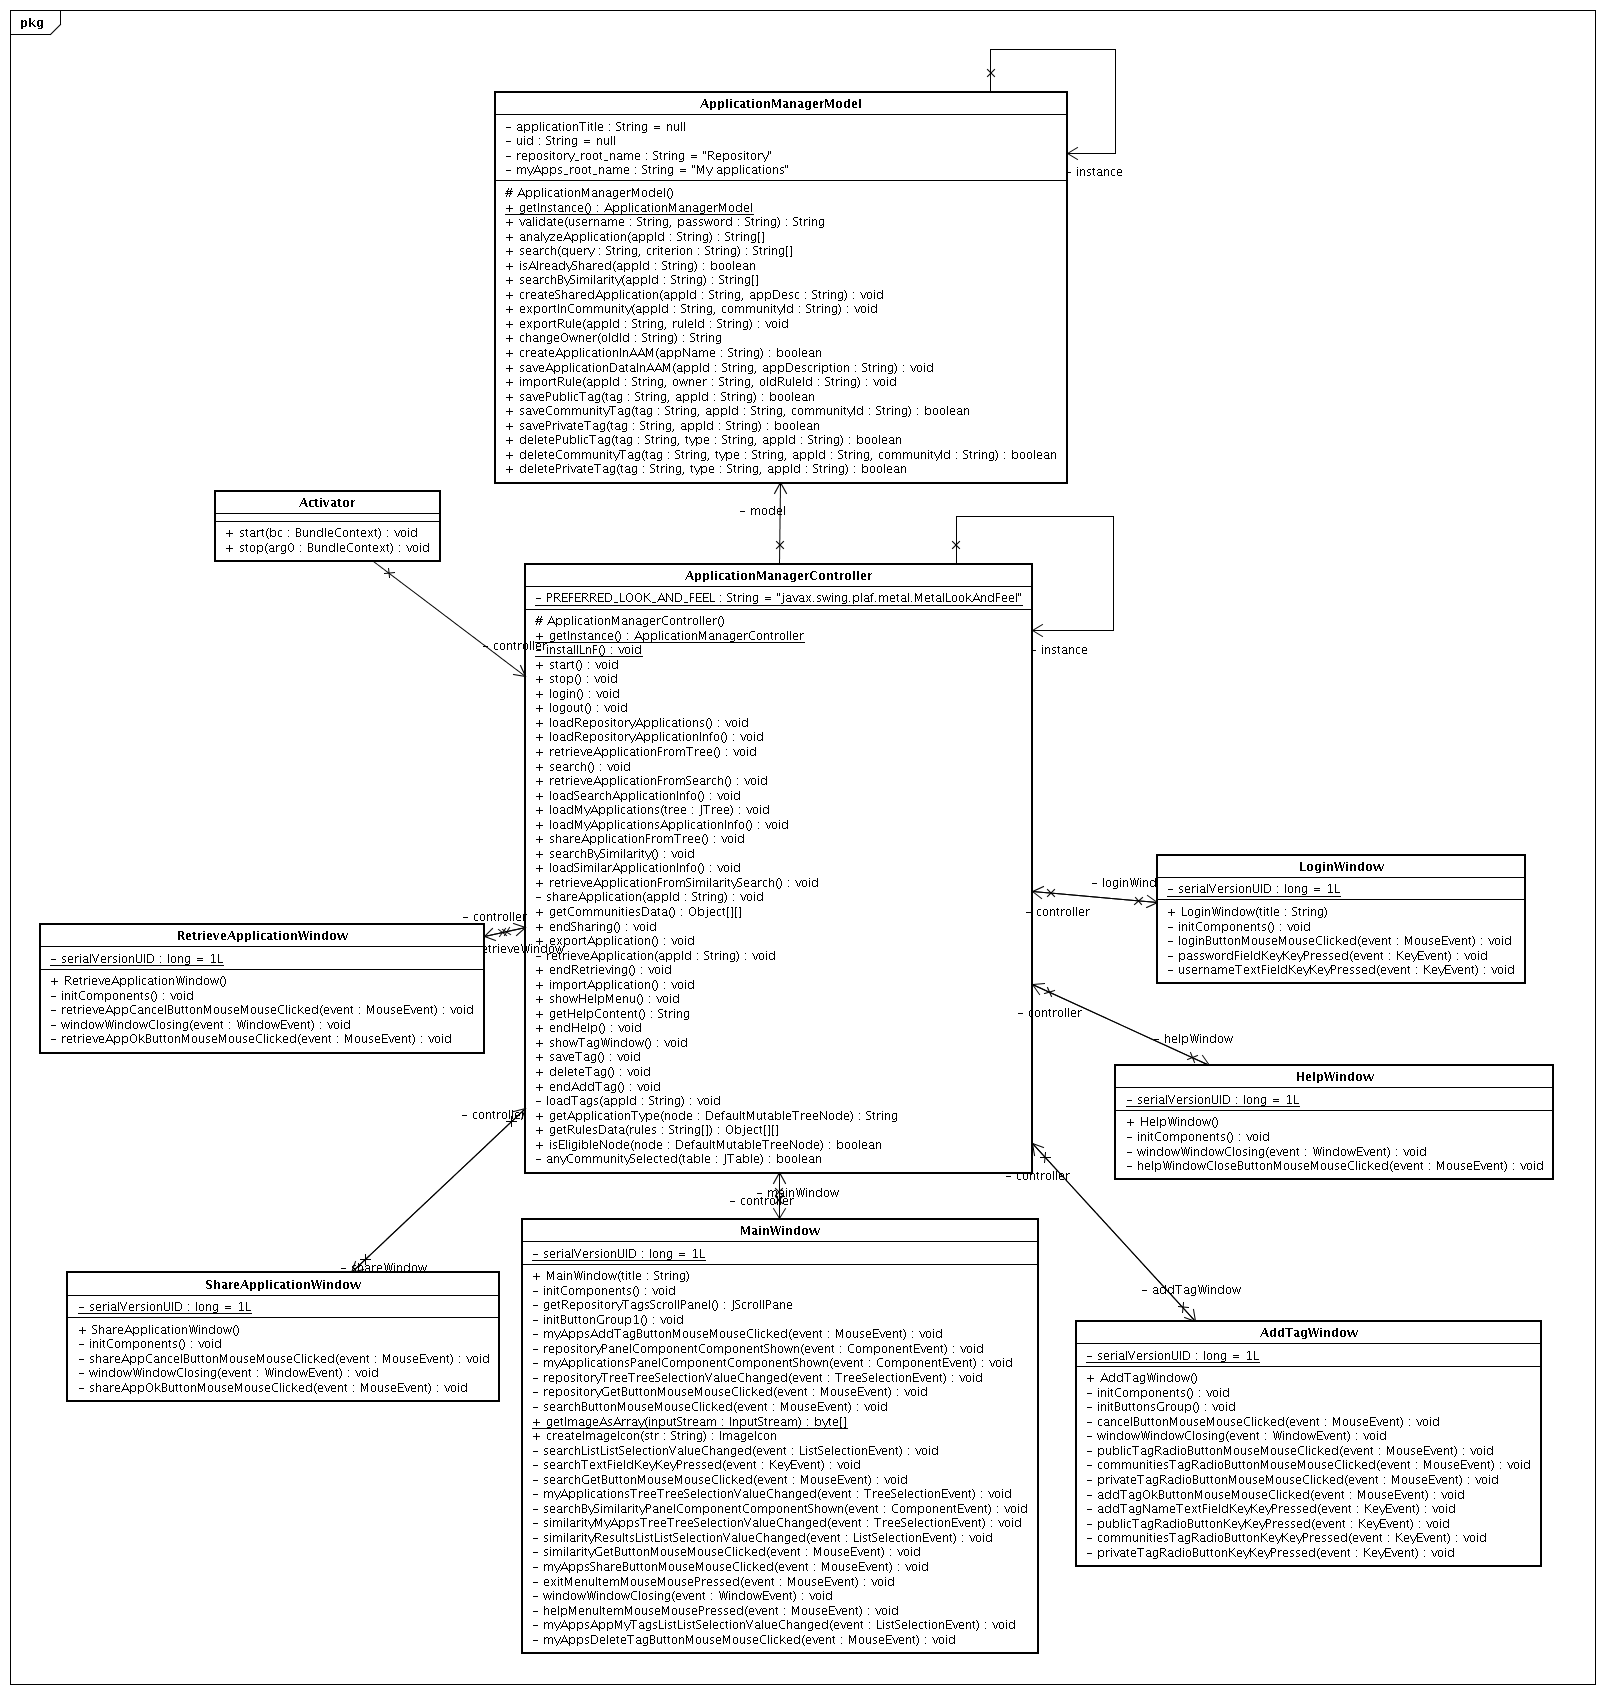
\includegraphics[scale=0.3]{diagrams/ApplicationManagerClassDiagramSmall.png}
  \caption{\label{img:am-cd}ApplicationManager (class diagram)}
 \end{center}
\end{figure}

\subsubsection{GUI design}

Finally, we need to decide the composition of the graphical user interface. It
was divided into the following windows:
\begin{itemize}
  	\item \verb|LoginWindow|: Displays a window where the user can introduce his
  	user name and password.
  	\item \verb|MainWindow|: Displays a window where the user can manage the
  	local and remote applications. It is divided into the following tabs:
	\begin{itemize}
  		\item ``My applications'': 
  			\begin{itemize}
		  		\item It allows the user to browse his applications, see the 
		  		information about them and share them in the repository.
		  		\item It allows the user to manage tags associated to certain 
		  		application.
              \end{itemize}
  		\item ``Repository'': It allows the user to browse the repository, to see
  		information about the applications and to retrieve them.
  		\item ``Search'': It allows the user to perform queries 
  		to look for applications in the repository by different criteria:
  		description, tags, type or any.
  		\item ``Search by similarity'': It allows the user to search
  		applications by choosing one he has in his local space.
    \end{itemize}
    It will also offer a menu tab with options to look up for remote help and
    to log out of the system.
    
    \item \verb|ShareApplicationWindow|: Displays a window where the user can
    customize the parameters of the sharing process: select the communities, 
    select the rules, visualize their description, etc.
    \item \verb|RetrieveApplicationWindow|: Displays a window where the user can
    customize the parameters of the retrieving process: select the rules,
    visualize their description, change the application description, etc.
    \item \verb|AddTagWindow|: Displays a window where the user can tag an
    application and define its visibility.
    \item \verb|HelpWindow|: Displays a window with the help information.
    

\end{itemize}

The user interaction through this GUI is detailed in Section
\ref{sec:user-interaction}.

